\section{Experiment}
In our experiments, we aim to answer the following research questions:
\textbf{RQ1:} Can \ourmethod achieve state-of-the-art performance on the KGQA tasks?
\textbf{RQ2:} Can the planning module of \ourmethod be integrated with other LLMs to improve their performance?
% \textbf{RQ3:} Can \ourmethod be finetuned and effectively transferred to other knowledge graphs?
\textbf{RQ3:} Can \ourmethod conduct faithful reasoning and generate interpretable reasoning results?


\subsection{Experiment Settings}
% % \begin{wraptable}{r}{.35\columnwidth}
\begin{table}[]
    \centering
    % \vspace{-3mm}
    \caption{Statistics of datasets.}
    \label{tab:dataset}
    % \resizebox{.35\columnwidth}{!}{%
    \begin{tabular}{@{}c|ccc@{}}
        \toprule
        Datasets & \#Train & \#Test & Max \#hop \\ \midrule
        WebQSP   & 2,826   & 1,628  & 2         \\
        CWQ      & 27,639  & 3,531  & 4         \\ \bottomrule
    \end{tabular}%
    % }
    % \vspace{-3mm}
% \end{wraptable} 
\end{table}
\noindent\textbf{Datasets.} 
We evaluate the reasoning ability of \ourmethod on two benchmark KGQA datasets: WebQuestionSP (WebQSP) \citep{yih2016value} and Complex WebQuestions (CWQ) \citep{talmor2018web}, which contain up to 4-hop questions. Freebase \citep{bollacker2008freebase} is the background knowledge graph for both datasets, which contains around 88 million entities, 20 thousand relations, and 126 million triples. The details of the datasets are described in \Cref{app:dataset}. 


\noindent\textbf{Baselines.} We compare \ourmethod with 21 baselines grouping into 5 categories: 1) Embedding-based methods, 2) Retrieval-augmented methods, 3) Semantic parsing methods, 4) LLMs, and 5) LLMs+KGs methods. The details of each baseline are described in \Cref{app:baselines}.

\noindent\textbf{Evaluation Metrics.} Following previous works, we use Hits@1 and F1 as the evaluation metrics. Hits@1 measures the proportion of questions whose top-1 predicted answer is correct. Since a question may correspond to multiple answers, F1 considers the coverage of all answers, which balances the precision and recall of the predicted answers.

\noindent\textbf{Implementations.} For \ourmethod, we use LLaMA2-Chat-7B \citep{touvron2023llama} as the LLM backbone, which is instruction finetuned on the training split of WebQSP and CWQ as well as Freebase for 3 epochs. We generate the top-3 relation paths using beam-search for each question. Since UniKGQA \citep{jiang2022unikgqa} and DECAF \citep{yu2022decaf} are state-of-the-art methods, we directly refer their results and those of the other baselines reported in their papers for comparisons. For LLMs, we use zero-shot prompting to conduct KGQA. The detailed settings are described in \Cref{app:settings}.

\begin{table}[]
    \centering
    \caption{Performance comparison with different baselines on the two KGQA datasets.}
      \vspace{-3mm}
    \label{tab:kgqa}
    \resizebox{.7\columnwidth}{!}{%
    \begin{tabular}{@{}c|llccc@{}}
        \toprule
        \multirow{2}{*}{Type}             & \multirow{2}{*}{Methods}                & \multicolumn{2}{c}{WebQSP}    & \multicolumn{2}{c}{CWQ}       \\ \cmidrule(l){3-6} 
                                          &                                         & Hits@1        & F1            & Hits@1        & F1            \\ \midrule
        \multirow{5}{*}{Embedding}        & KV-Mem \citep{miller2016key}            & 46.7          & 34.5          & 18.4          & 15.7          \\
                                          & EmbedKGQA \citep{saxena2020improving}   & 66.6          & -             & 45.9          & -             \\
                                          & NSM \citep{he2021improving}             & 68.7          & 62.8          & 47.6          & 42.4          \\
                                          & TransferNet \citep{shi2021transfernet}  & 71.4          & -             & 48.6          & -             \\
                                          & KGT5 \cite{saxena2022sequence}          & 56.1          & -             & 36.5          & -             \\ \midrule
        \multirow{4}{*}{Retrieval}        & GraftNet \citep{sun2018open}            & 66.4          & 60.4          & 36.8          & 32.7          \\
                                          & PullNet \citep{sun2019pullnet}          & 68.1          & -             & 45.9          & -             \\
                                          & SR+NSM \citep{zhang2022subgraph}        & 68.9          & 64.1          & 50.2          & 47.1          \\
                                          & SR+NSM+E2E \citep{zhang2022subgraph}    & 69.5          & 64.1          & 49.3          & 46.3          \\ \midrule
        \multirow{4}{*}{Semantic Parsing} & SPARQL \citep{sun2020sparqa}            & -             & -             & 31.6          & -             \\
                                          & QGG \citep{lan2020query}                & 73.0          & 73.8          & 36.9          & 37.4          \\
                                          & ArcaneQA \citep{gu2022arcaneqa}         & -             & 75.3          & -             & -             \\
                                          & RnG-KBQA \citep{ye2022rng}              & -             & 76.2          & -             & -             \\ \midrule
        \multirow{5}{*}{LLMs}             & Flan-T5-xl \citep{chung2022scaling}     & 31.0          & -             & 14.7          & -             \\
                                          & Alpaca-7B \citep{taoristanford}         & 51.8          & -             & 27.4          & -             \\
                                          & LLaMA2-Chat-7B \citep{touvron2023llama} & 64.4          & -             & 34.6          & -             \\
                                          & ChatGPT                                 & 66.8          & -             & 39.9          & -             \\
                                          & ChatGPT+CoT                             & 75.6          & -             & 48.9          & -             \\ \midrule
        \multirow{4}{*}{LLMs+KGs}         & KD-CoT \citep{wang2023knowledge}        & 68.6          & 52.5          & 55.7          & -             \\
                                          & UniKGQA \citep{jiang2022unikgqa}        & 77.2          & 72.2          & 51.2          & 49.1          \\
                                          & DECAF (DPR+FiD-3B) \citep{yu2022decaf}  & 82.1          & \textbf{78.8} & -             & -             \\ \cmidrule(l){2-6} 
                                          & \ourmethod             & \textbf{85.7} & 70.8          & \textbf{62.6} & \textbf{56.2} \\ \bottomrule
        \end{tabular}   
    }
    \vspace{-6mm}
\end{table}


\subsection{RQ1: KGQA Performance Comparison}
\noindent\textbf{Main Results.} In this section, we compare \ourmethod with other baselines on KGQA tasks. The results are shown in \Cref{tab:kgqa}. Our method achieves the best performance on both datasets across most metrics. Specifically, compared to the SOTA method DECAF~\citep{yu2022decaf} on WebQSP, our method improves Hits@1 by 4.4\%. On the CWQ dataset, which is more challenging due to multi-hop questions, our method improves both Hits@1 and F1 by 22.3\% and 14.4\% against the SOTA model UniKGQA~\citep{jiang2022unikgqa}. These results demonstrate the superior reasoning ability of our method in KGQA.

Among other methods, retrieval-augmented approaches outperform conventional embedding-based methods by retrieving relevant subgraphs from KGs, which reduces reasoning complexity. Furthermore, SR+NSM and SR+NSM+E2E adopt relation paths-based retrieval which achieves better performance, highlighting the importance of relation paths.
%
Semantic parsing methods perform better than retrieval methods on WebQSP but worse on CWQ due to the complexity of generating logical queries for complex questions in CWQ. Although LLMs-based methods achieve comparable performance, they are limited by hallucinations and lack of knowledge as shown in \Cref{sec:cases}. The LLMs+KGs methods achieve the second-best performance, which demonstrates the effectiveness of unifying KGs and LLMs for reasoning.

\textbf{Ablation Study.} We conduct an ablation study to analyze the effectiveness of the \emph{planning module} and \emph{reasoning module} in our method (\ourmethod). We compare four variants: 1) \emph{w/o planning}, where we remove the planning module and perform reasoning without retrieved reasoning paths; 2) \emph{w/o reasoning}, where we remove the reasoning module and use all answers from retrieved reasoning paths as results; 3) \emph{w/ random plans}, where we randomly retrieve reasoning paths from KGs and feed them into the reasoning module; 4) \emph{w/ vote reasoning}, where we adopt the majority voting to select top-5 answers from retrieved reasoning paths. The results are shown in \Cref{tab:ablation}.

% \begin{table}[]
\begin{wraptable}{r}{.6\columnwidth}
    \centering
    \vspace{-5mm}
    \caption{Ablation studies of \ourmethod.}
      \vspace{-3mm}
    \label{tab:ablation}
    \resizebox{.6\columnwidth}{!}{%
    \begin{tabular}{@{}l|ccc|ccc@{}}
        \toprule
        \multirow{2}{*}{Method}    & \multicolumn{3}{c|}{WebQSP} & \multicolumn{3}{c}{CWQ}                                                                     \\ \cmidrule(l){2-7}
                                   & Precision                   & Recall                  & F1             & Precision      & Recall         & F1             \\ \midrule
        \ourmethod                 & \textbf{74.77}              & 75.84                   & \textbf{70.81} & \textbf{57.69} & 58.19          & \textbf{56.17} \\ \midrule
        \ourmethod w/o planning    & 57.26                       & 50.16                   & 49.69          & 35.35          & 34.77          & 33.76          \\
        \ourmethod w/o reasoning   & 46.90                       & \textbf{79.85}          & 49.56         & 18.88         & \textbf{67.89} & 22.26          \\\midrule
        \ourmethod w/ random plans & 38.66                       & 38.31                   & 35.24          & 38.99          & 39.29          & 37.64          \\ 
        \ourmethod w/ vote reasoning & 54.80	& 60.44	& 47.96	& 22.92	& 47.98	& 26.52 \\ 
        \bottomrule
    \end{tabular}%
    }
    \vspace{-4mm}
\end{wraptable} 
% \end{table}


From the results, it is evident that without a planning module, our method degenerates to conventional LLMs that solely rely on questions as input, suffering from the lack of knowledge issue. Although removing the reasoning module leads to high recall due to an increased number of answers, precision drops significantly because of noise in retrieved paths. This demonstrates the effectiveness of the reasoning module in identifying important reasoning paths and filtering out noise. Furthermore, using random plans achieves worse performance than removing the planning module, highlighting the importance of a planning module who generates faithful reasoning plans. Using a simple majority vote reasoning can improve the results which also demonstrate the necessity of reasoning module.

\begin{figure}[]
    \begin{center}
    %\framebox[4.0in]{$\;$}
    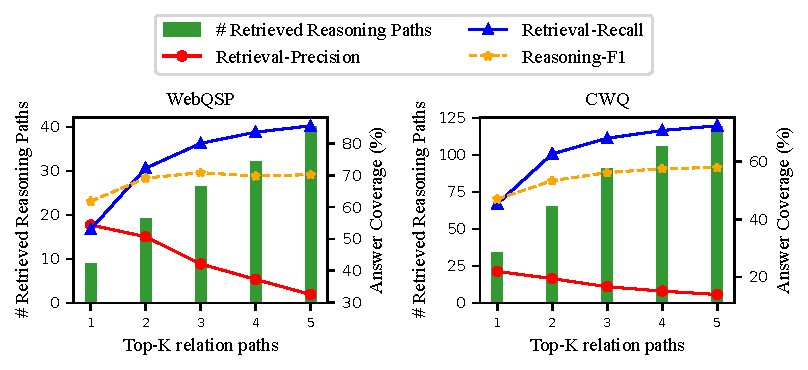
\includegraphics[width=0.7\columnwidth,trim=0 2mm 0 0,clip]{images/k-beam.pdf}
    \end{center}
    \vspace{-4mm}
    \caption{Faithfulness of top-$K$ generated relation paths. \emph{Green bars} denote the average number of retrieved reasoning paths, \emph{solid lines} denote the answer coverage of the retrieved paths, and \emph{dashed line} denote the answer coverage of the reasoning module based on the retrieved reasoning paths.}
    \label{fig:k-beam}
    \vspace{-7mm}
\end{figure}

\subsection{RQ2: Plug-and-Play \ourmethod Planning Module}
% \begin{table}[]
\begin{wraptable}{r}{.5\columnwidth}
    \centering
    \vspace{-4mm}
    \caption{Effects of integrating the planning module of \ourmethod with different LLMs for reasoning.}
    \vspace{-3mm}
    \label{tab:plug-and-play}
    \resizebox{.5\columnwidth}{!}{%
    \begin{tabular}{@{}lcccc@{}}
        \toprule
        \multirow{2}{*}{Methods} & \multicolumn{2}{c}{WebQSP} & \multicolumn{2}{c}{CWQ}                                   \\ \cmidrule(l){2-5}
                                 & Hits@1                     & Recall                  & Hits@1         & Recall         \\ \midrule
        ChatGPT                  & 66.77                      & 49.27                   & 39.90          & 35.07          \\
        ChatGPT + \ourmethod Planning              & \textbf{81.51}             & \textbf{71.60}          & \textbf{52.68} & \textbf{48.51} \\ \midrule
        Alpaca-7B                & 51.78                      & 33.65                   & 27.44          & 23.62          \\
        Alpaca-7B + \ourmethod Planning              & \textbf{56.16}             & \textbf{74.20}          & \textbf{44.04} & \textbf{38.46} \\ \midrule
        LLaMA2-Chat-7B           & 64.37                      & 44.61                   & 34.60          & 29.91          \\
        LLaMA2-Chat-7B + \ourmethod Planning      & \textbf{74.20}             & \textbf{56.16}          & \textbf{56.41} & \textbf{51.99} \\ \midrule
        Flan-T5-xl                  & 30.95                      & 17.08                   & 14.69          & 12.25          \\
        Flan-T5-xl + \ourmethod Planning             & \textbf{67.87}             & \textbf{44.93}          & \textbf{37.81} & \textbf{32.57} \\ \bottomrule
    \end{tabular}
    }
    \vspace{-4mm}
\end{wraptable} 
% \end{table}
In this section, we evaluate the effectiveness of integrating the planning module of \ourmethod with different LLMs during inference to improve their performance. Specifically, we first adopt the planning module of \ourmethod to generate relation paths and feed the retrieved reasoning paths as context into different LLMs for reasoning. The results are presented in \Cref{tab:plug-and-play}. To account for the fact that it is difficult to extract the number of answers from LLM's output. We only report the Hits@1 and Recall metrics. 

From the results, we can notice that the performance of all LLMs is substantially improved by integrating the planning module of \ourmethod. Specifically, the Hits@1 of ChatGPT, Alpaca, LLaMA2, and Flan-T5 are improved by 8.5\%, 15.3\%, and 119.3\%, respectively. This demonstrates that the planning module of \ourmethod can be seamlessly integrated with other LLMs to improve their performance without retraining.

% \begin{table}
    \centering
    \caption{Performance of \ourmethod on MetaQA-3hop.}
    \label{tab:transfer}
    %\resizebox{2.2in}{!}{%
    \begin{tabular}{@{}l|cc@{}}
        \toprule
        \multirow{3}{*}{Strategies}         & \multicolumn{2}{c}{MetaQA-3hop}                  \\ \cmidrule(l){2-3}
                                            & Hits@1                          & F1             \\ \midrule
        \ourmethod (train from scratch)  & 84.81                           & 41.32          \\
        \ourmethod (transfer from Freebase) & \textbf{88.98}                  & \textbf{50.68} \\ \bottomrule
    \end{tabular}
    %}
\end{table} 


\begin{table}
    \centering
    \RE{
    \caption{Training time comparison.}
    \label{tab:time}
    %\resizebox{2.2in}{!}{%
    \begin{tabular}{@{}c|cc@{}}
        \toprule
        Method & Training on Freebase & Transferring to Wiki-Movies \\
        \midrule
        \ourmethod & 38 hours & 2 hours \\
        \bottomrule
    \end{tabular}
    %}
    }
\end{table} 

% \subsection{RQ3: Transferability to Other KGs}
% We also evaluate the transferability of \ourmethod to other KGs. We select the MetaQA-3hop dataset \citep{zhang2018variational} which is based on Wiki-Movies KGs\footnote{\url{https://research.fb.com/downloads/babi.}}. We select 1000 samples from the training split and utilize two training strategies to finetune \ourmethod: 1) \emph{training from scratch}, where we directly optimize \ourmethod with 1000 samples; 2) \emph{transfer from Freebase}, where we conduct a further finetuning based on \ourmethod trained for Freebase. The results are shown in \Cref{tab:transfer}. From results, we can see that transfer from Freebase achieves better performance than training from scratch, which demonstrates the transferability of \ourmethod to other KGs.

\subsection{RQ3: Faithful reasoning and interpretable results}\label{sec:cases}
\noindent\textbf{Quantitative Results.} To evaluate the faithfulness of the relation paths, we illustrate the quantitative results in \Cref{fig:k-beam}. In experiments, we sweep the number of top-$K$ relation paths generated by \ourmethod. From results, we can see that the number of retrieved reasoning paths increases with $K$, which also leads to more answers to be covered (recall). This demonstrates the faithfulness of the relation paths by retrieving the answers. However, more retrieved reasoning paths also lead to more noise and retrieval time (shown in \Cref{app:retrieval_cost}), which decreases the precision and makes little contribution to the final results (reasoning-f1). Therefore, we set $K=3$ in experiments.


\begin{table}[]
    \centering
    \caption{Example of \textit{lack of knowledge} for ChatGPT-CoT and interpretable predictions of \ourmethod.}
    \vspace{-3mm}
    \label{tab:case1}
    \resizebox{.7\columnwidth}{!}{%
    \begin{tabular}{@{}c|p{5in}@{}}
        \toprule
        Question             & What type of government is used in the country with Northern District?                                                                                                                                                                                                                                                                                               \\ \midrule
        Answer               & Parliamentary system                                                                                                                                                                                                                                                                                                                                                 \\ \midrule
        ChatGPT + CoT        & To determine what type of government is used in a country with a Northern District, \textcolor{red}{we need more specific information}. The term "Northern District" does not specify the name of any particular country or provide enough context to identify its government type. \textcolor{red}{Could you please provide additional details or clarify the specific country you are referring to?} \\ \midrule
        Reasoning Paths      & Northern District $\to$ location.administrative\_division.first\_level\_division\_of $\to$ Israel $\to$ government.form\_of\_government.countries $\to$ \textbf{Parliamentary system}                                                                                                                                                                                         \\
        \midrule
        \ourmethod & \begin{tabular}[c]{@{}p{5in}@{}}The type of government used in the country with the Northern District is a \textbf{Parliamentary system}.\\\\  Explanations:\\ \\ 1. Northern District $\to$ location.administrative\_division.first\_level\_division\_of $\to$ Israel: \\ The Northern District is a part of Israel.\\ 2. Israel $\to$ government.form\_of\_government.countries $\to$ Parliamentary system: Israel has a Parliamentary system of government.\\ \\ So, by following the reasoning paths provided, we can conclude that the country with the Northern District, which is Israel, uses a Parliamentary system of government.\end{tabular}                                                                                                                                                                                                                                                                                                                                            \\ \bottomrule
    \end{tabular}}
    \vspace{-3mm}
\end{table}


\begin{table}[]
    \centering
    \caption{Example of the \textit{hallucination} of ChatGPT-CoT and faithful reasoning of \ourmethod.}
    \vspace{-3mm}
    \label{tab:case2}
    \resizebox{.7\columnwidth}{!}{%
    \begin{tabular}{@{}c|p{5in}@{}}
        \toprule
        Question             & Where is the home stadium of the team who won the 1946 World Series championship?
        \\ \midrule
        Answer               & Busch Stadium                                                                                                                                                                                                                                                                                                                                                 \\ \midrule
        ChatGPT + CoT        & \begin{tabular}[c]{@{}p{5in}@{}}Step 1: Identify the team that won the 1946 World Series championship.
            The team that won the 1946 World Series championship was the St. Louis Cardinals. \\\\
            
            Step 2: Determine the home stadium of the St. Louis Cardinals during that time. The St. Louis Cardinals' home stadium during the 1946 season was  \textcolor{red}{Sportsman's Park}. \\\\
            
            Therefore, the possible answer to the question "Where is the home stadium of the team who won the 1946 World Series championship?" is:
            -  \textcolor{red}{Sportsman's Park}.\end{tabular}
             \\ \midrule
        Reasoning Paths      & \begin{tabular}[c]{@{}p{5in}@{}} 1946 World Series $\to$ sports.sports\_team.championships $\to$ St. Louis Cardinals $\to$ sports.sports\_team.arena\_stadium $\to$ \textbf{Busch Stadium}\\
            1946 World Series $\to$ sports.sports\_team.championships $\to$ St. Louis Cardinals $\to$ sports.sports\_team.arena\_stadium $\to$ \textcolor{red}{Roger Dean Stadium}\end{tabular}\\
        \midrule
        \ourmethod & \begin{tabular}[c]{@{}p{5in}@{}}Based on the reasoning paths provided, the home stadium of the team who won the 1946 World Series championship is \textbf{Busch Stadium}. This conclusion is based on the following path:\\\\

            \textbf{1. 1946 World Series $\to$ sports.sports\_team.championships $\to$ St. Louis Cardinals $\to$ sports.sports\_team.arena\_stadium $\to$ Busch Stadium} \\\\
            
            The reasoning path leads us to the St. Louis Cardinals as the team that won the 1946 World Series, and Busch Stadium is the stadium associated with the St. Louis Cardinals. Therefore, \textbf{Busch Stadium} is the home stadium of the team that won the 1946 World Series championship.\end{tabular}                                                                                                                                                                                                                                                                                                                                            \\ \bottomrule
    \end{tabular}}
    \vspace{-5mm}
\end{table}

\noindent\textbf{Case studies.} We also illustrate two case studies in \Cref{tab:case1} and \Cref{tab:case2}. In \Cref{tab:case1}, we can find that ChatGPT+CoT suffers from the lack of knowledge issue and cannot answer the question. On the contrary, \ourmethod can generate faithful relation paths and retrieve valid reasoning paths from KGs for reasoning. Besides, \ourmethod can provide interpretable explanations based on the reasoning paths. In \Cref{tab:case2}, we can see that ChatGPT+CoT suffers from hallucinations and generates incorrect answers. In contrast, although the retrieved reasoning paths contain noises, the reasoning module can identify the correct reasoning paths and conduct faithful reasoning. These results demonstrate the effectiveness of \ourmethod in conducting faithful reasoning and generating interpretable results. More cases can be found in \Cref{app:case_rel,app:case_inter}.

